%
% 3_Arrokoth.tex
%
% (c) 2020 Prof Dr Andreas Müller, Hochschule Rapperswil
%
% !TEX root = ../../buch.tex
% !TEX encoding = UTF-8
%
\section{Arrokoth
\label{planet:section:arrokoth}}
\rhead{Arrokoth}

Arrokoth, abgebildet in \cref{planet:fig:arrokoth}, ist ein kleiner Asteroid aus dem Kuipergürtel, der auch unter der ursprünglichen Bezeichnung (486958) und 2014 \(\text{MU}_{69}\) bekannt ist.
Der Name Arrokoth ist Powhatan/Algonquianisch und heisst „Himmel“.

Arrokoth ist das am weitesten entfernte Objekt, das jemals mit einer Raumsonde erforscht wurde.
Es wurde mit Hilfe des Hubble Weltraum Teleskops 2014 vom New Horizons Wissenschaftsteam entdeckt und als Ziel für die Erforschung durch die New Horizons Sonde ausgewählt.
Die Informationen zu Arrokoth sind von \cite{planet:arrokoth} entnommen.

Solche „Weltraumschneemänner“ können nur entstehen, wenn die eigene Gravitation kleiner ist als die starren Kräfte des Körpers.
Das bedeutet die Himmelskörper sind kleinere Objekte im Vergleich zu Planeten.
Zusätzlich dazu dürfen die einzelnen Asteroiden nicht mit grossen Kräften aufeinander treffen, das bedeutet das Verbinden der zwei Körper geschieht relativ langsam.
Wenn zwei Asteroiden mit grosser Geschwindigkeit aufeinander treffen, würden sie in kleinere Trümmer zerschmettert werden, die über längeren Zeitraum wieder einen Asteroiden bilden, der wiederum eine Kugelform hat.

\begin{figure}[h]
    \centering
    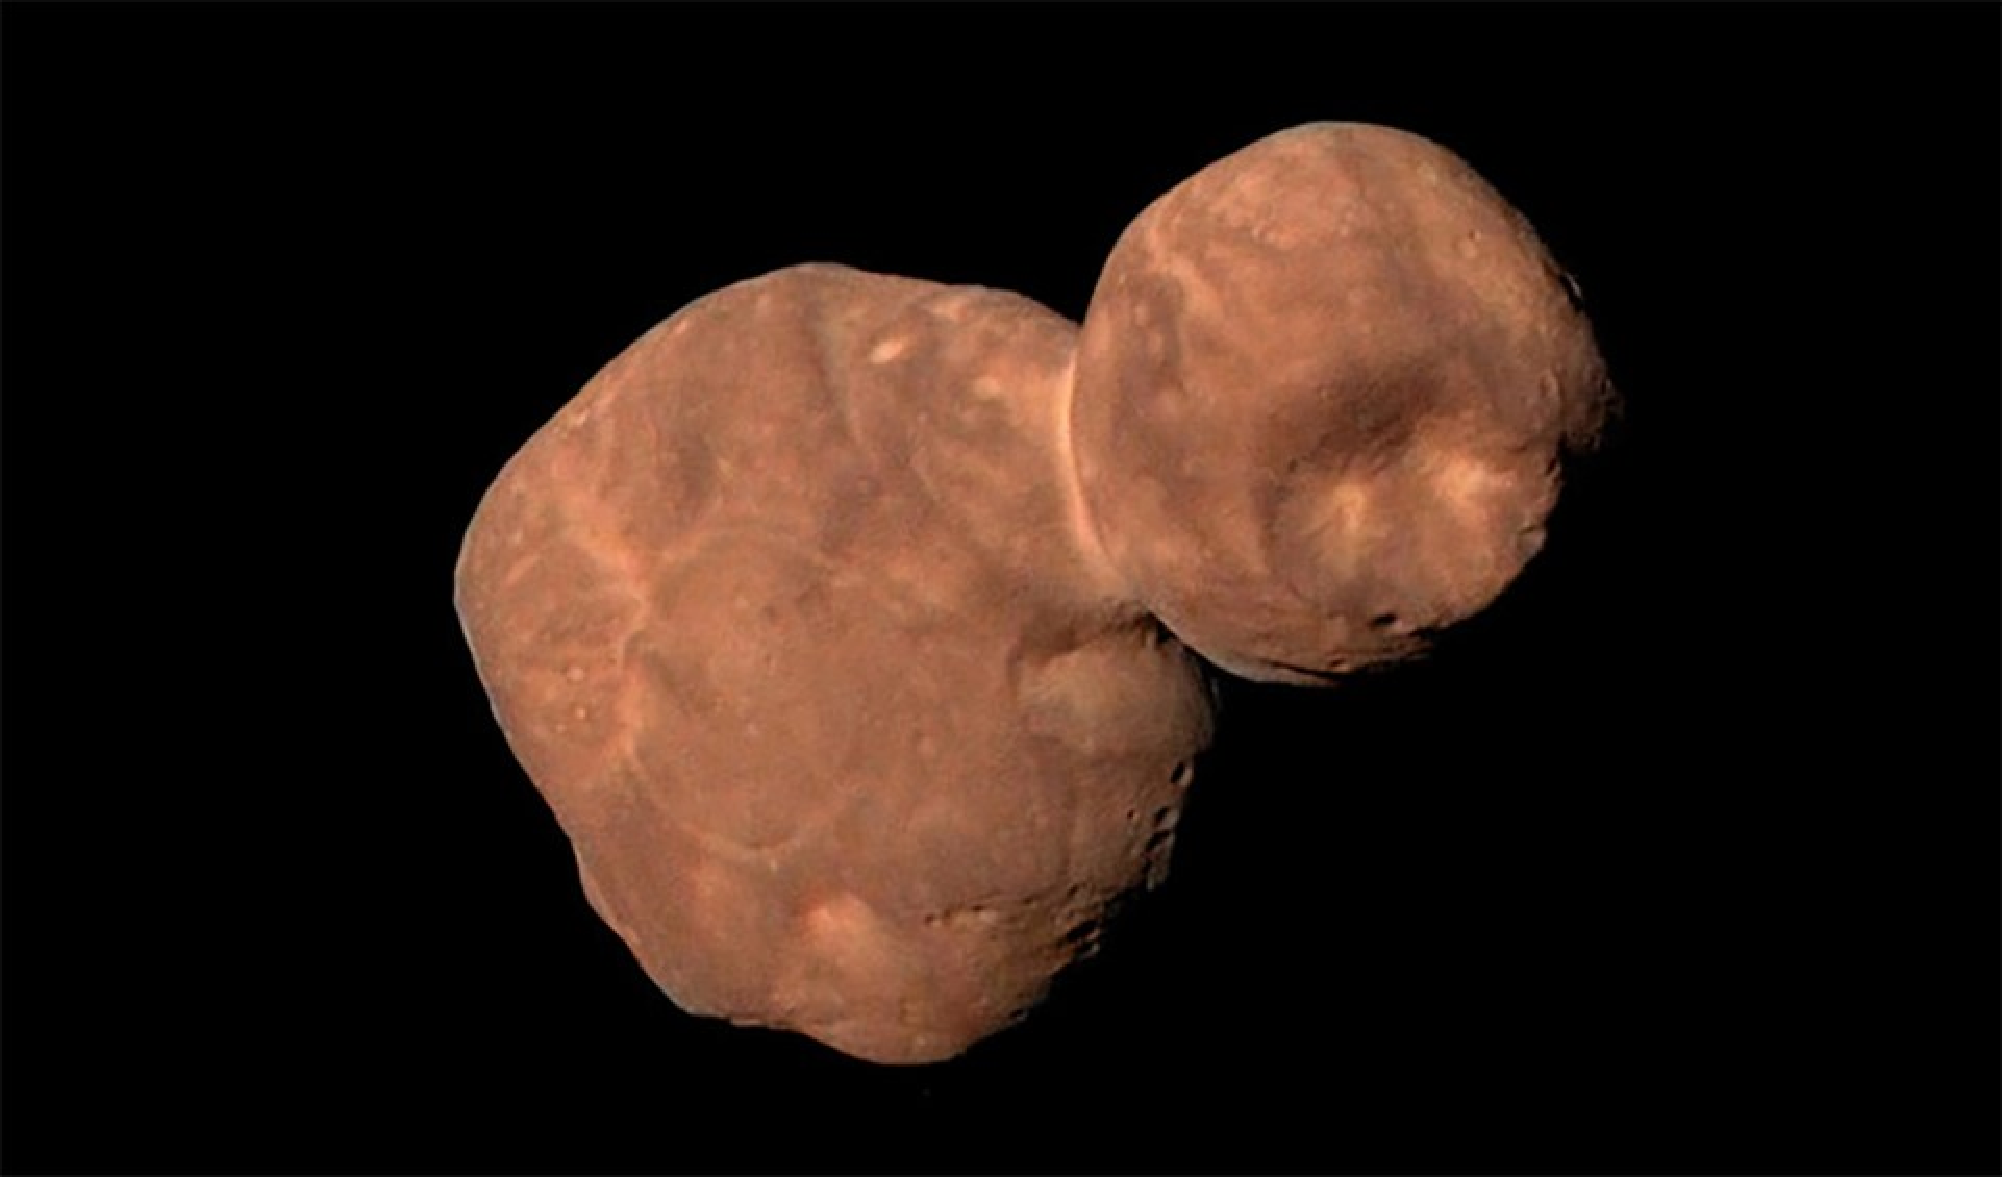
\includegraphics[width=\linewidth]{papers/planet/pictures/Arrokoth.pdf}
    \caption{Arrokoth aus dem Kuipergürtel \cite{planet:arrokothpic}
        \label{planet:fig:arrokoth}}
\end{figure}